\chapter{Background and Motivation} \label{chap:chap-1}

% if you want a short header you can use the following command
% \chapter[short-header-name]{chapter-title} \label{chap:chap-1}


% add your chapter text here
\section{Electrochemistry}
Given the pivotal role of reduction-oxidation (redox) reactions in materials chemistry and industrial applications, electrochemistry stands as a primary beneficiary of advancements in SDLs. According to the broad definition commonly accepted among researchers, electrochemistry encompasses the study of both the physical and chemical characteristics of ionic conductors, along with phenomena taking place at the interfaces between these ionic conductors and electronic conductors, semiconductors, other ionic conductors, and even insulating materials (such as gases and vacuum) \cite{Bagotsky2005}. The flow of electrons only occurs between two species, but the transfer of charge can also occur through an oxidation-reduction reaction. When a substance loses an electron, its oxidation state increases, indicating oxidation. When a substance acquires an electron, its oxidation state decreases, indicating reduction. For example, consider the following redox reaction, which has oxidation and reduction components:
\begin{align}
H\textsubscript{2} + F\textsubscript{2} \to 2HF \label{eq:reaction} \\
H\textsubscript{2} \to 2H\textsuperscript{+} + 2e\textsuperscript{-} \quad \text{Oxidation} \label{eq:oxidation}\\
F\textsubscript{2} + 2e\textsuperscript{-} \to 2F\textsuperscript{-} \quad 
\text{Reduction} \label{eq:reduction}
\end{align}
A redox reaction is balanced when the number of electrons gained by the oxidant is equal to the number of electrons lost by the reductant. Like any balanced chemical equation, the entire process is electrically neutral, meaning that the net charge remains consistent on both sides of the equation.
With redox reactions, it is possible to separate the oxidation and reduction half-reactions physically in space, provided a complete circuit exists using an external electrical link, such as a wire, connecting the two halves. Electrons migrate from the reductant to the oxidant as the reaction progresses through this electrical connection, generating an electric current. 

Devices that use redox reactions to generate electricity or use electricity to drive non-spontaneous redox reactions are called electrochemical cells. This device effectively transforms chemical energy into electrical energy or vice-versa. In an electrochemical cell, reduction and oxidation reactions occur at the electrodes. The electrode where reduction occurs is termed the cathode, while oxidation occurs at the anode. An electrode serves as a stable electrical conductor, facilitating the flow of electrical current within non-metallic solids, liquids, gases, plasmas, or even vacuums. Electrodes are typically fabricated from highly conductive materials, including but limited to metals and graphite \cite{goldbook}. In a battery, redox reactions create a flow of electrical current that can be used to power electronic devices.

Electrode potential is the voltage of an electrochemical cell composed of a reference electrode and another electrode to be characterized.
\begin{figure}[h!]
  \centering
    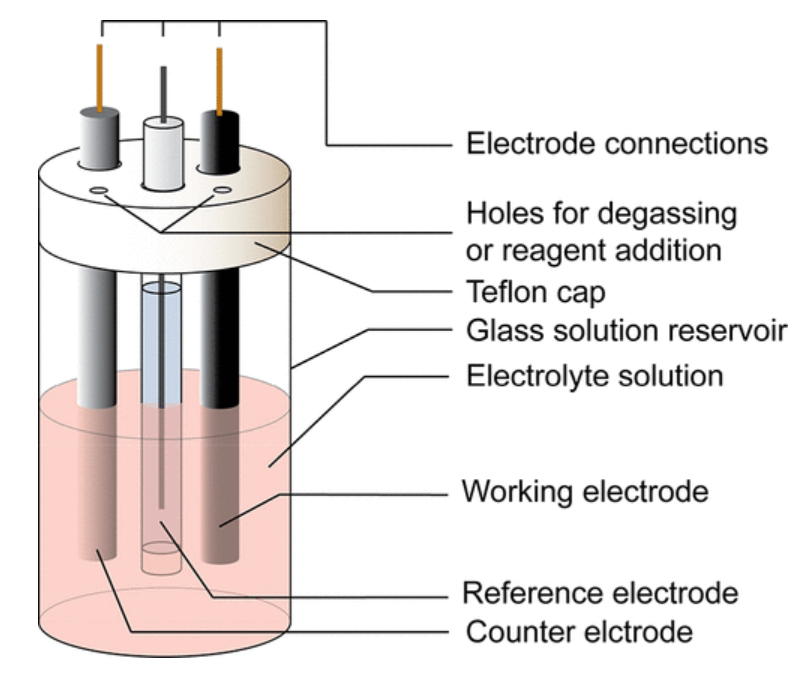
\includegraphics[width=0.8\textwidth]{figures/cv_diagram.png}
    \caption{Schematic of Electrochemical Cell \cite{Elgrishi2018}}
    \label{cell_schematic}
\end{figure}
Figure \ref{cell_schematic} shows a three-electrode setup typical for electrochemical experiments such as cyclic voltammetry. During the flow of current between the working and counter electrodes, the reference electrode is used to precisely measure the applied potential in relation to a stable reference reaction.
\begin{figure}[h!]
  \centering
    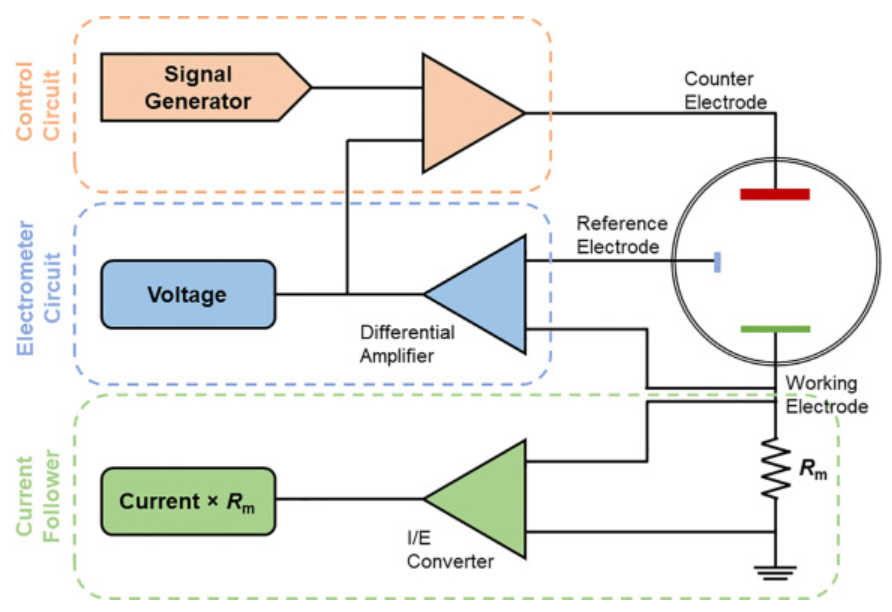
\includegraphics[width=1.0\textwidth]{figures/potentiostat_diagram.png}
    \caption{Potentiostat Circuit Diagram}
    \label{potentiostat_diagram}
\end{figure}
A potentiostat, as shown in Figure \ref{potentiostat_diagram}, is an analytical instrument designed to control the potential between the working electrode and counter electrode within a multi-electrode cell \cite{Zoski2006-zx}. The potentiostat contains various internal circuits tailored to fulfil this role, facilitating the generation and measurement of potentials and currents. External wires within a cell cable establish connections between the potentiostat circuit and the electrodes within the electrochemical cell. In a three-electrode configuration, the cell cable links the working, counter, and reference electrodes on one terminal and the potentiostat cell cable connector on the opposite end. The potentiostat's internal circuitry governs the applied signal. 

The working electrode performs the electrochemical event of interest. Since reactions occur at the cathode and anode surfaces, it is crucial that the surface is spotless and that the surface area is well-defined. The working electrodes should be immediately polished after use to ensure there are no surface contaminants that inhibit electron transfer. Even a few hours of air exposure will degrade the electrode surface. Detecting when surface contamination affects data quality is one of the questions this work addresses. This detection can trigger automatic polishing or replacement with a new disposable electrode \cite{Yoshikawa2024}.

Commercial vendors commonly provide potentiostats that are governed by proprietary software, employ graphical user interfaces (GUI), and produce already curated data. These devices are widely used for electroanalytical experiments such as cyclic voltammetry and differential pulse voltammetry. Commercial potentiostats can vary in design, but a typical potentiostat is shown in Figure \ref{potentiostat_diagram} and consists of three component circuits: a control circuit, an electrometer, and a current follower \cite{WAIN20211}. The electrometer circuit utilizes a differential amplifier to measure the difference in potential between the working and reference electrodes. Subsequently, the measured potential feeds into the control circuit, which administers a current through the counter electrode, altering the relative potential of the working electrode to align with the user-defined parameters. A single generator ensures this potential adheres to a predefined periodic waveform. The current flowing through the working electrode is then assessed by a current follower circuit, commonly in the form of a current-to-voltage converter. This circuit measures the drop in potential across a grounded resistor, allowing the current to be determined using Ohm's law.

However, commercial potentiostats present challenges for integration into automated systems due to their reliance on proprietary software and GUIs. Furthermore, their high cost poses a significant barrier for groups seeking to perform high-throughput analysis.

To address these issues, Pablo-García et al. recently introduced an open-source, low-cost potentiostat \cite{PabloGarca2024}. This innovative device aims to democratize electrochemical analysis by reducing the financial barrier to entry and improving integration with automation systems. By providing an affordable and accessible alternative to traditional commercial potentiostats, this open-source solution empowers researchers to conduct electrochemical experiments with greater flexibility and efficiency. Despite its remarkable advancements, the device's precision falls short of commercial standards. As such, we later explore various machine-learning methodologies to enhance data quality. 
\section{Cyclic Voltammetry}
\begin{figure}[h!]
  \centering
    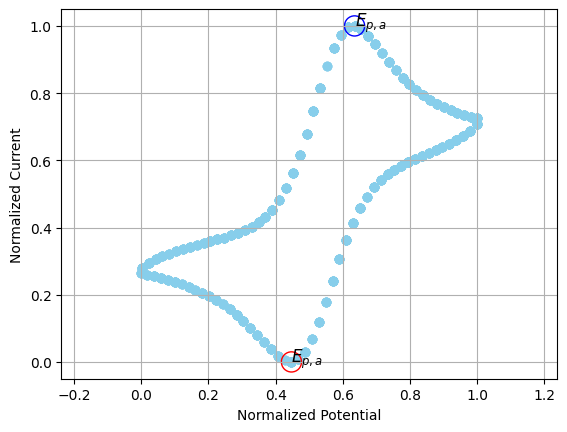
\includegraphics[width=1.0\textwidth]{figures/cv_example.png}
    \caption{Cyclic Voltammogram}
    \label{cv_example}
\end{figure}
Cyclic voltammetry (CV) is a common electrochemical characterization that extracts important reduction and oxidation information about molecules \cite{doi:10.1021/ac60210a007}. Typically, the working electrode potential increases linearly with time. After reaching a predetermined limit, the potential decreases to return to the starting voltage. These cycles can be repeated as frequently as needed to bolster confidence in the obtained data. The rate of voltage change over time is known as the experiment's scan rate \mbox{(Voltage/Time)} and affects how many data points are gathered throughout the experiment \cite{https://doi.org/10.1002/anie.198408313}. 

CV is valuable for studying qualitative information about electrochemical processes across diverse conditions. It enables the examination of intermediates in oxidation-reduction reactions and the assessment of reaction reversibility. Other use cases include the determination of electron stoichiometry, analyte diffusion coefficients, and formal reduction potentials, aiding in identification processes \cite{Nicholson1964}. Additionally, in reversible Nernstian systems, the proportional relationship between concentration and current allows for determining unknown solution concentrations by constructing calibration curves correlating current and concentration \cite{Libretexts_2023}.

In a typical cyclic voltammogram shown in Figure \ref{cv_example}, peaks represent electrochemical processes occurring at the electrode surface. The anodic peak ($\mathrm{E_{p, a}}$) is observed during the scan where oxidation of the electroactive species occurs at the electrode and corresponds to the potential at which oxidation is most favourable. The current increases as the potential applied to the electrode becomes more positive, reaching a maximum at the peak potential. The cathodic peak ($\mathrm{E_{p, c}}$) is observed during the reverse scan where reduction of the electroactive species occurs at the working electrode and corresponds to the potential at which reduction is most favorable. The current increases as the potential becomes more negative, reaching a maximum at the peak potential \cite{GRIMSHAW20001}. Typically, chemists are especially interested in these peaks as they condense the redox behavior of the analyzed compound \cite{Faulkner1983}.
\section{Differential Pulse Voltammetry}
\begin{figure}[h!]
  \centering
    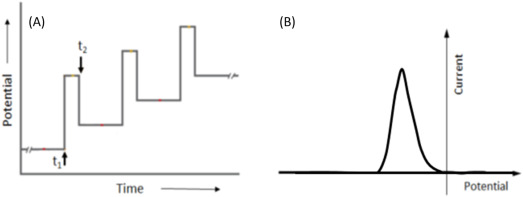
\includegraphics[width=1.0\textwidth]{figures/dpv.jpg}
    \caption{Differential Pulse Voltammogram}
    \label{dpv_example}
\end{figure}
Differential Pulse Voltammetry (DPV) is a more sophisticated electrochemical measurement technique where a series of increasing pulses are applied across the electrodes in an electrochemical cell \cite{Scholz2005-pa}. The current $I_1$ is measured right before applying the pulse at time $t_1$, and $I_2$ is measured again at the end at time $t_2$. The difference in current ($\Delta I_2 - I_1$) is plotted against the potential and results in a peak-like shape. 
This method helps reduce the impact of charging current by sampling the current just before the potential change. DPV is well suited for measurements with extremely low concentrations of chemicals. This is because the effect of the charging current can be minimized to achieve high sensitivity, and only the faradaic current, the electric current generated by the redox of a chemical at an electrode, is extracted so that electrode reactions can be measured precisely \cite{Laborda2014}. 

Furthermore, DPV is a versatile tool for the qualitatively characterizing chemical compounds and their electrochemical properties \cite{Scholz2005-pa}. By analyzing the shape, position, and area of the peaks in the DPV curve, chemists can glean insights into the nature of the electroactive species present, their concentration, kinetics of electron transfer processes, and other relevant electrochemical parameters. This capability makes DPV invaluable in various fields such as analytical chemistry, environmental monitoring, and pharmaceutical research, where understanding the behaviour of chemical compounds at the molecular level is crucial \cite{Scholz2005-pa}.